\documentclass[a4paper,12pt]{article}
\usepackage[utf8]{inputenc}
\usepackage{amssymb,amsmath,uniinput,graphicx,hyperref, multirow,siunitx}
\usepackage[section]{placeins}
\usepackage[ngerman]{babel}
\usepackage[left=3cm,right=3cm,top=3cm,bottom=3cm]{geometry}
\renewcommand{\familydefault}{\sfdefault}
\setlength{\belowcaptionskip}{6pt}
\hypersetup{pdfinfo = {
	Title={Versuchsprotokoll zu Positronen im Festkörper},
	Author={Knut Kiesel, Tobias Pook},
	Keywords={Teilchenfalle}
}}


\graphicspath{ {../pictures/} }
\title{Laborpraktikum Teilchenphysik\\ Lebensdauer von Positronen im Festkörper}
\author{Knut Kiesel\\Tobias Pook}
\date{\today}

\begin{document}
\maketitle
\vspace{5cm}
\tableofcontents
\thispagestyle{empty}
\newpage
\setcounter{page}{1}

\section{Ziel des Versuches}
Ziel des Versuches ist der Aufbau und die Inbetriebnahme einer Messstation,
die in der Lage ist die Lebensdauer von Positronen in Festkörpern in der
Größenordnung von $\si{ps}$ zu messen.

Hierzu wird $^{22}$Na verwendet, welches beim Zerfall in $^{22}$Ne
zuerst ein γ-Quant der Energie $1.28\si{MeV}$ abgibt und dann ein Positron emittiert.
Nach einer vom Festkörper abhängigen Zeit annihiliert das Positron unter Aussendung
von 2 bis 3 γ Quanten mit einer Energie von $0.511\si{keV}$.
Durch das messen der Zeitdifferenz zwischen dem ersten γ-Quant des Übergangs und dem
γ aus der Annihilation kann die Lebensdauer des Positrons bestimmt werden.



\section{Aufbau und Durchführung}
%Kommentare aus der Vorbesprechung:
%	Constant Fraction Discriminator liefert logisches out bei BLD Ausgang
%	Die Delay Einheit ändert die polarität des Signal, wenn gewünscht.
%	Der Multi Channel Analyzer nimmt nur positive Signal ohne Offset an.

Der Detektor besteht aus zwei zylindrischen Szintiallatonsdetektoren, welche in einem Gehäuse
mit einem Photomultiplier verbaut sind. Die radioaktiven Proben werden zwischen beiden Szintillatoren
platziert. Die Photomultiplier werden mit einer Spannung von $2\si{kV}$ betrieben. Von beiden Photomultipliern
wird sowohl das Anodensignal als auch das Dynodensignal abgegriffen und für das Messen und Triggern der 
Zeitabstandsmessung genutzt. Hierbei liefert jeweils ein Photomultiplier das Start und der andere 
das Stoppsignal für die Zeitmessung liefert.
Die elektronische Signalverabreitung unterteilt sich in zwei Schaltkreise: \\
\begin{itemize}
	\item
	Ein "langsamer Kreis" dieser prüft ob die gemessenen Photonen sich im richtigen Energieintervall 
	befinden und erzeugt abhängig davon ein Triggersignal.
	\item Ein "schneller Kreis" dieser bestimmt die Zeitdifferenz und gibt dieses in Form eines Pulses an einen
	Vielkananlanalysator weiter, sofern ein Triggersignal vom "langsamen Kreis" besteht.	
\end{itemize}
\subsection*{langsamer Kreis}
	Für den langsamen Kreis wird das Dynodensiganl der Photomultiplier genutzt und in jeweils einem 
	Einzelkanaldiskriminator weiter verarbeitet, dieser verstärkt das Signal zunächst (es wird
	ein Gain von 300 eingestellt). 
	% Erklären was beim Differenzieren passiert.
	
\begin{figure}[htb]
		\centering
		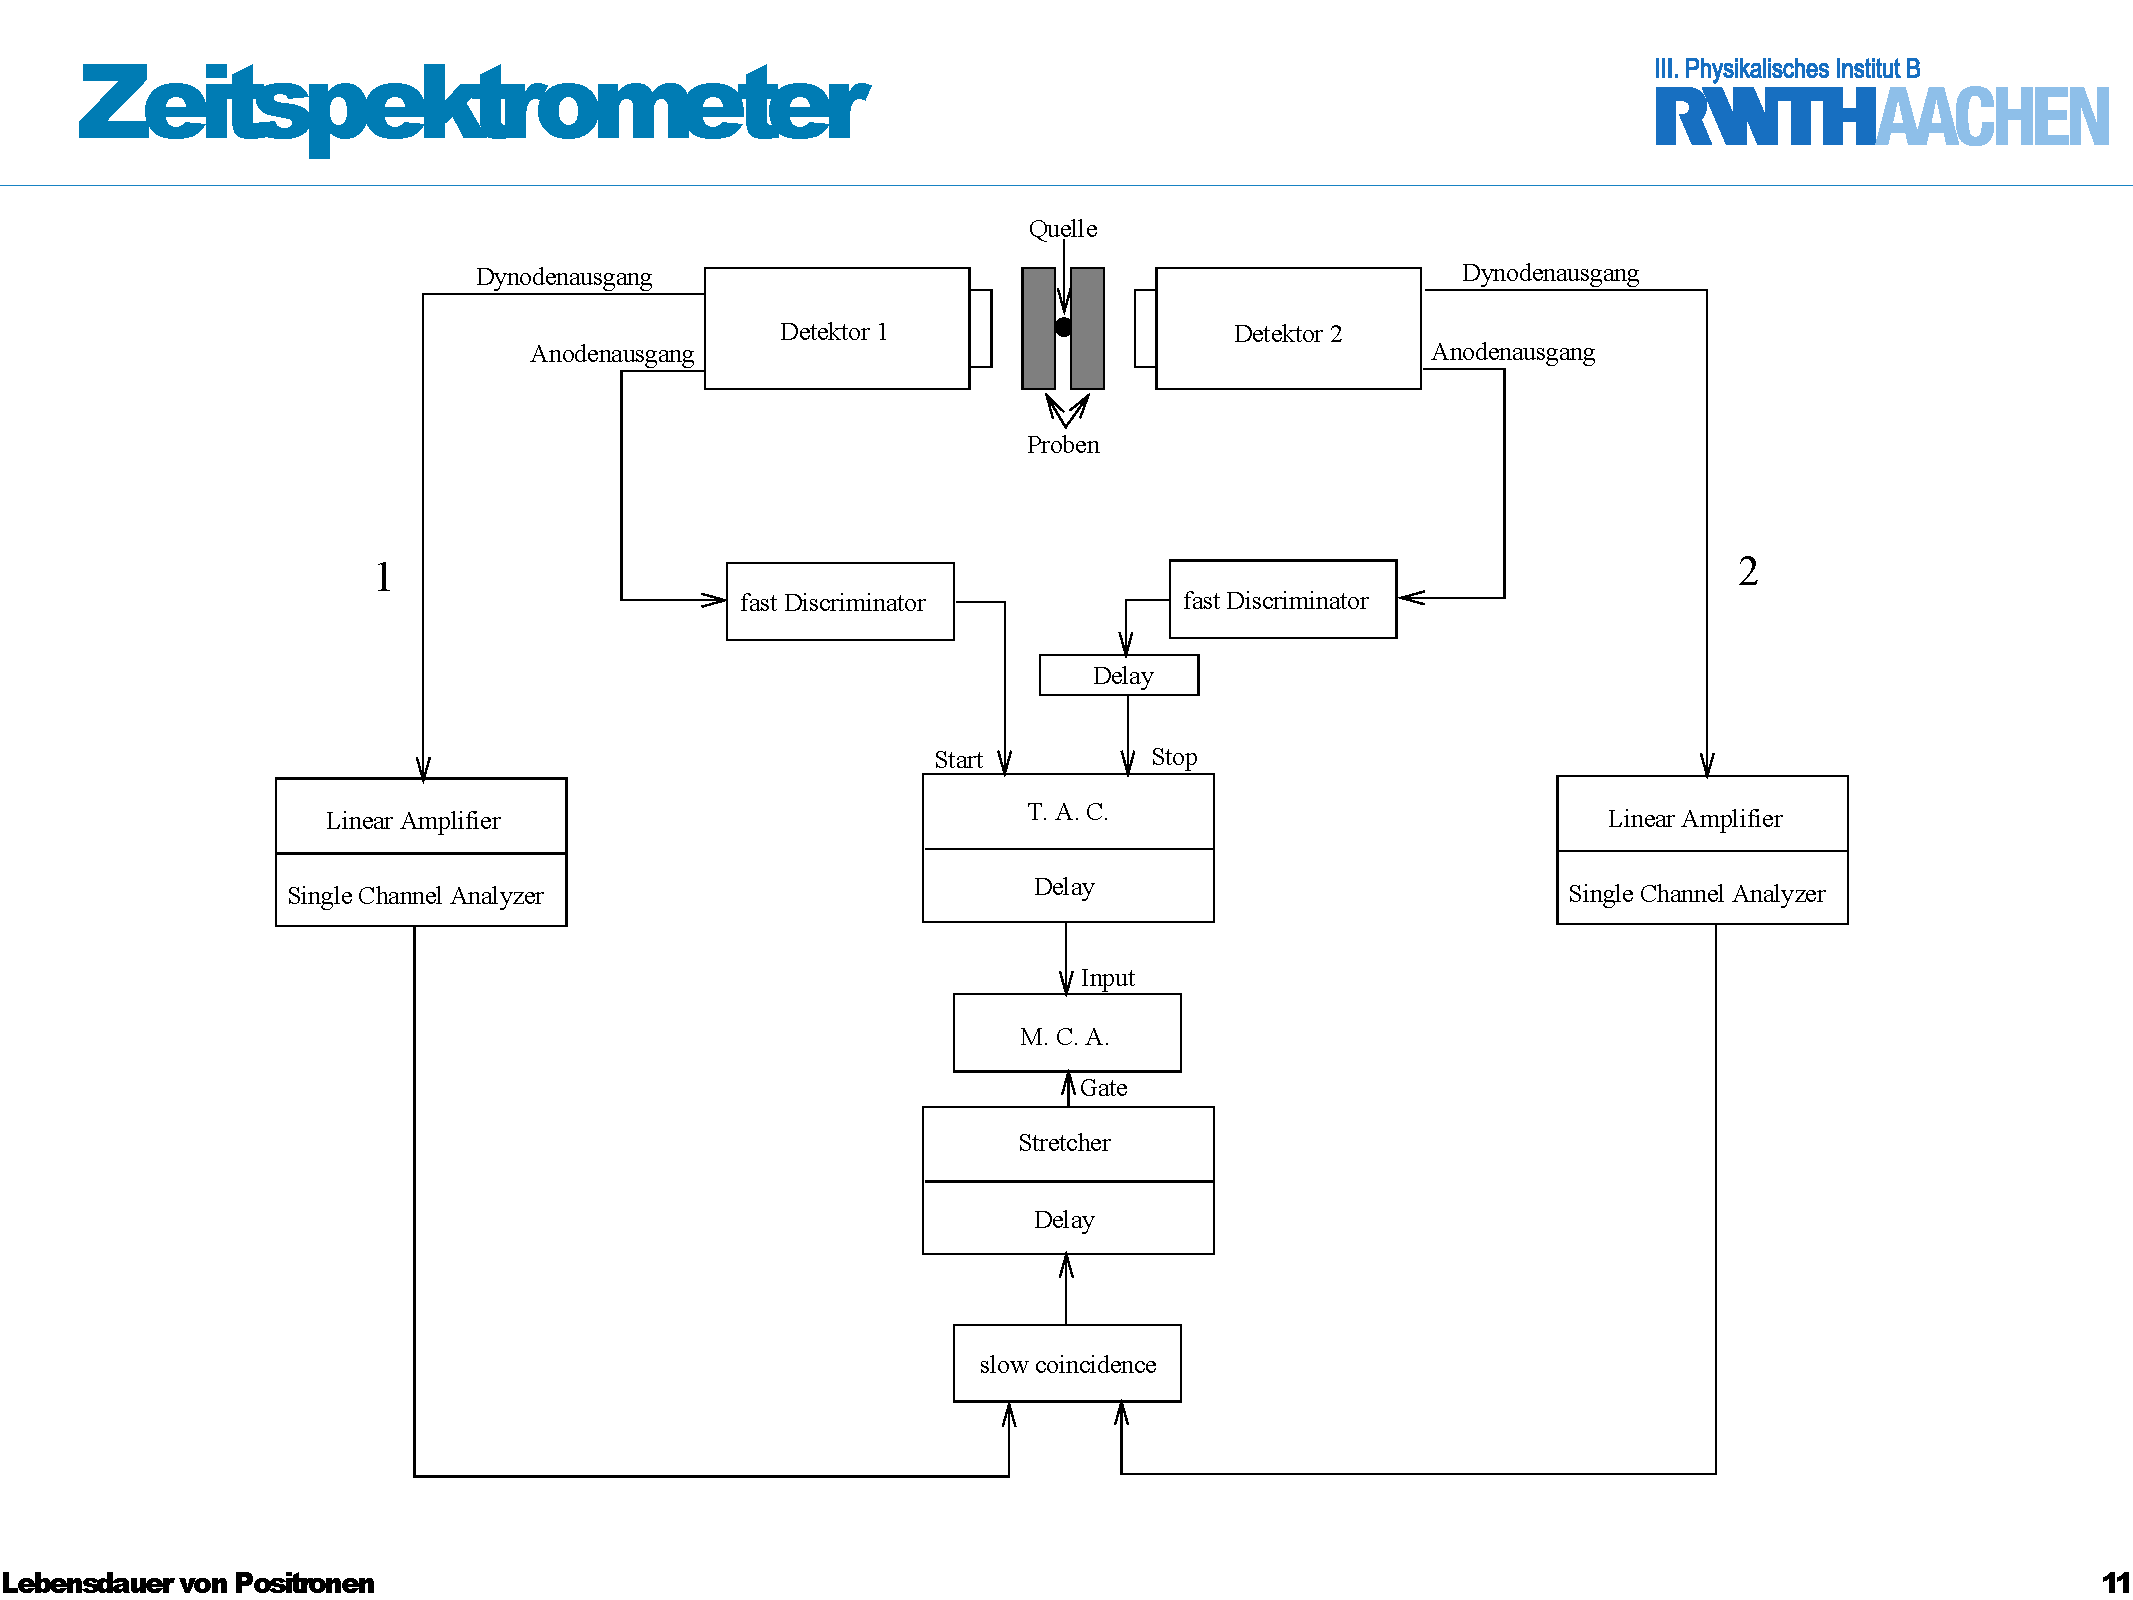
\includegraphics[width=0.8\textwidth]{schaltplan.pdf}
		\caption{Schaltplan}
		\label{fig:schaltplan}
\end{figure}
\section{Ergebnisse}

\section{Diskussion}
\end{document}
